\section{Evaluation}
\label{sec:evaluation}

\begin{table*}[t]
\centering
\resizebox{\textwidth}{!}{
\begin{tabular}{ |c|c|c|c|c|c|c|c|c|c|c|c|c| } 
 \hline
  &  & \multicolumn{2}{|c|}{\textbf{25, 25 samples}} & \multicolumn{2}{|c|}{\textbf{100, 100 samples}} & \multicolumn{2}{|c|}{\textbf{250, 250 samples}} & \multicolumn{2}{|c|}{\textbf{500, 500 samples}} & \multicolumn{2}{|c|}{\textbf{1000, 1000 samples}} \\ \hline
Clustering & true loss & \# queries & estimated loss & \# queries & estimated loss & \# queries & estimated loss & \# queries & estimated loss  & \# queries & estimated loss \\ \hline
C1 (single) & \textbf{0.06107} & 51 &	0.06 & 204	& 0.025 & 519 &	0.028 & 1023 &	0.024 & 2070 &	0.028 \\ \hline
C2 (complete) &	\textbf{0.04177} &	50 & 0.02 &	210 &	0.005 & 514 &	0.018 &		1024 &	0.016 &		2056 &	0.015   \\ \hline
C3 (weighted) & \textbf{0.03831} &	50 & 0.02 &	203 &	0.015 &	518 &	0.008 &		1027 &	0.016 &		2057 &	0.018  \\ \hline
C4 (average) &	\textbf{0.03489} &	52 & 0.02 &	207 &	0.020 &	519	&   0.008 &		1043 &	0.013 &		2061 &	0.014   \\ \hline
\end{tabular}
}
\caption{Simulated dataset: Impact of number of samples on the loss of the clustering}
\label{tab:exp1}
\end{table*}

\begin{table*}[t]
\centering
\resizebox{\textwidth}{!}{
\begin{tabular}{ |c|c|c|c|c|c|c|c|c|c|c|c|c| } 
 \hline
  &  & \multicolumn{2}{|c|}{\textbf{25, 25 samples}} & \multicolumn{2}{|c|}{\textbf{100, 100 samples}} & \multicolumn{2}{|c|}{\textbf{250, 250 samples}} & \multicolumn{2}{|c|}{\textbf{500, 500 samples}} & \multicolumn{2}{|c|}{\textbf{1000, 1000 samples}} \\ \hline
Clustering & true loss & \# queries & estimated loss & \# queries & estimated loss & \# queries & estimated loss & \# queries & estimated loss  & \# queries & estimated loss \\ \hline
C1 (single) & \textbf{0.11075} & 51	& 0.08 & 208 &	0.055 &		516 &	0.054 &		1031 &	0.041 &		2079 &	0.046 \\ \hline
C2 (complete) &	\textbf{0.37172} &	50 & 0.34 &	204 &	0.315 &	510 &	0.348 &		1035 &	0.334 &		2070 &	0.343   \\ \hline
C3 (weighted) & \textbf{0.29622} &	51 & 0.14 &	203 &	0.260 &	521 &	0.236 &		1037 &	0.239 &		2071 &	0.229  \\ \hline
C4 (average) &	\textbf{0.26877} &	50 & 0.20 &	204 &	0.195 &	518 &	0.188 &		1027 &	0.202 &		2074 &	0.193   \\ \hline
\end{tabular}
}
\caption{Publications dataset: Impact of number of samples on the loss of the clustering}
\label{tab:exp2}
\end{table*}

\begin{figure*}[t]
    \centering
    \begin{subfigure}[t]{0.22\textwidth}
        \centering
        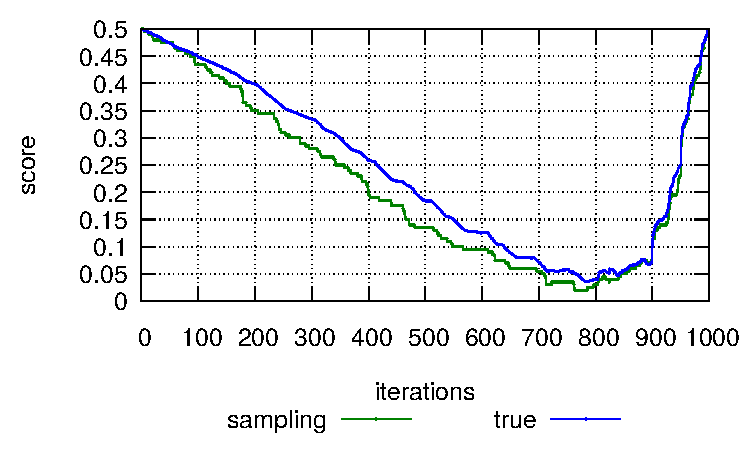
\includegraphics[height=3.2cm, width=4.2cm,valign=t]{figures/plot_simulated_s.pdf}
        \caption{Single linkage}
    \end{subfigure}%
    ~ 
    \begin{subfigure}[t]{0.22\textwidth}
        \centering
        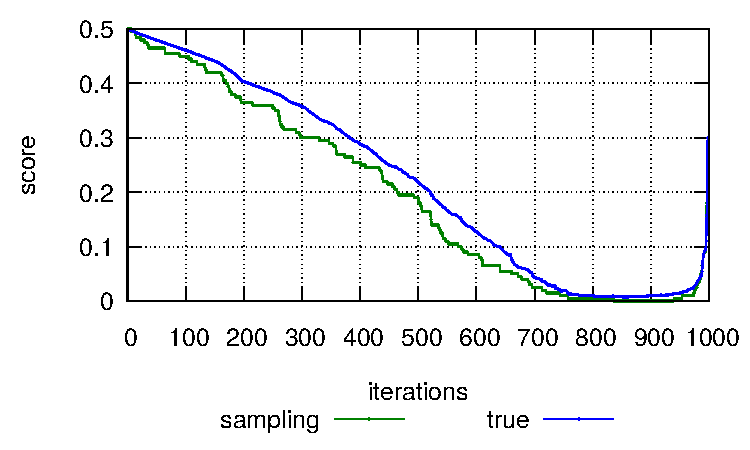
\includegraphics[height=3.2cm, width=4.2cm,valign=t]{figures/plot_simulated_c.pdf}
        \caption{Complete linkage}
    \end{subfigure}
	~
	\begin{subfigure}[t]{0.22\textwidth}
        \centering
        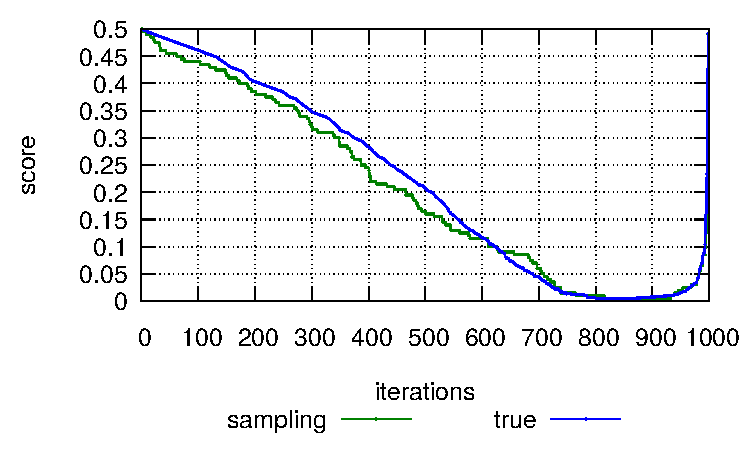
\includegraphics[height=3.2cm, width=4.2cm,valign=t]{figures/plot_simulated_w.pdf}
        \caption{Weighted linkage}
    \end{subfigure}
    ~
	\begin{subfigure}[t]{0.22\textwidth}
        \centering
        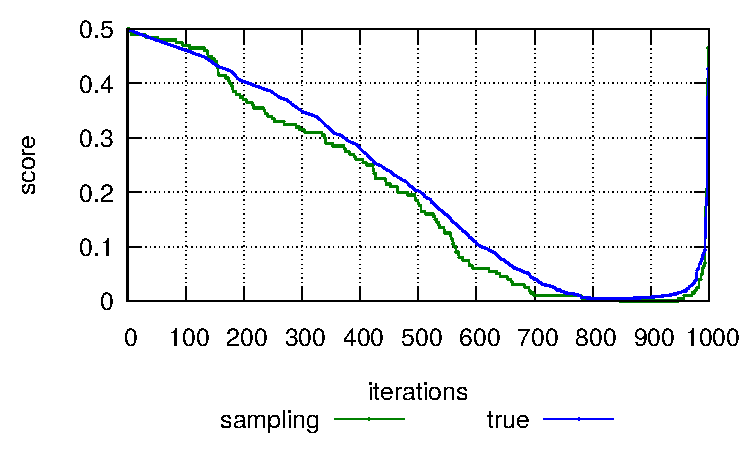
\includegraphics[height=3.2cm, width=4.2cm,valign=t]{figures/plot_simulated_a.pdf}
        \caption{Average linkage}
    \end{subfigure}
    
    \caption{Simulated dataset: Loss reported for every iteration of hierarchical clustering}
    \label{fig:simulated}
\end{figure*}

\begin{figure*}[t]
    \centering
    \begin{subfigure}[t]{0.22\textwidth}
        \centering
        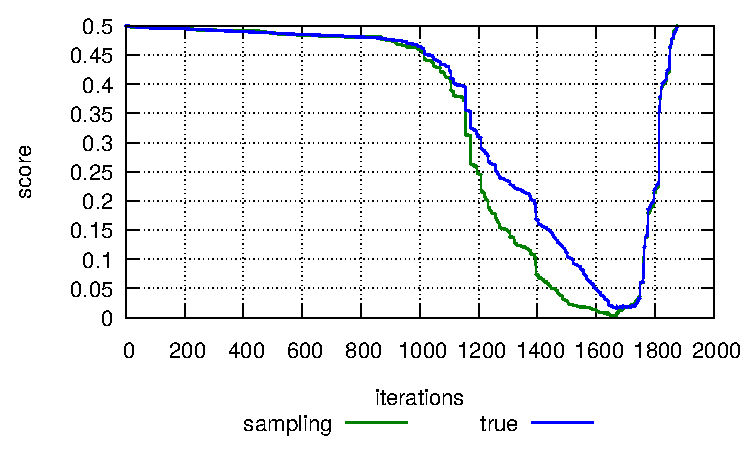
\includegraphics[height=3.2cm, width=4.2cm,valign=t]{figures/plot_real_s.pdf}
        \caption{Single linkage}
    \end{subfigure}%
    ~ 
    \begin{subfigure}[t]{0.22\textwidth}
        \centering
        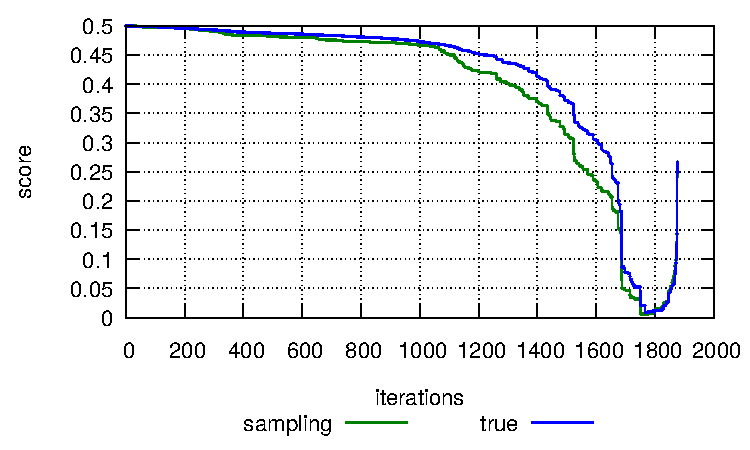
\includegraphics[height=3.2cm, width=4.2cm,valign=t]{figures/plot_real_c.pdf}
        \caption{Complete linkage}
    \end{subfigure}
	~
	\begin{subfigure}[t]{0.22\textwidth}
        \centering
        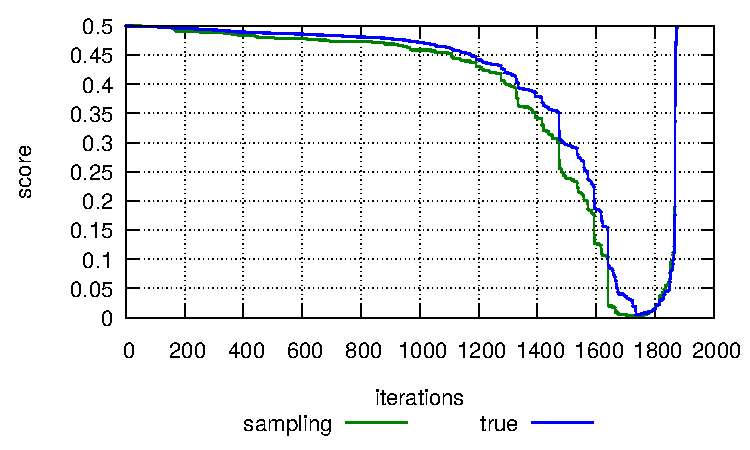
\includegraphics[height=3.2cm, width=4.2cm,valign=t]{figures/plot_real_w.pdf}
        \caption{Weighted linkage}
    \end{subfigure}
    ~
	\begin{subfigure}[t]{0.22\textwidth}
        \centering
        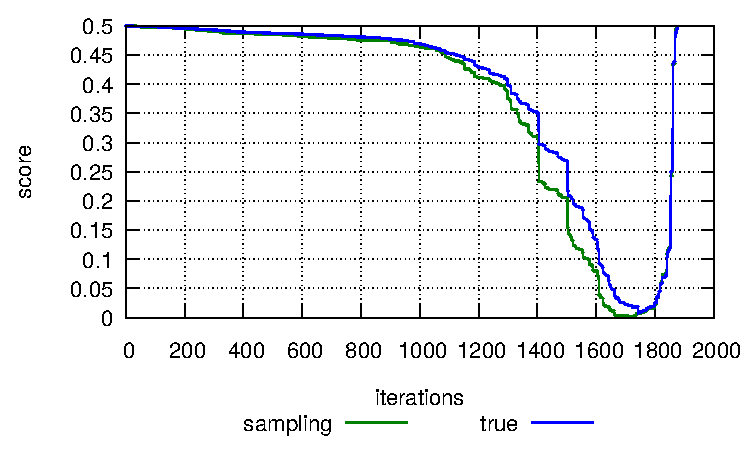
\includegraphics[height=3.2cm, width=4.2cm,valign=t]{figures/plot_real_a.pdf}
        \caption{Average linkage}
    \end{subfigure}
    
    \caption{Publications dataset: Loss reported for every iteration of hierarchical clustering}
    \label{fig:publications}
\end{figure*}

\begin{table}[t]
\centering
\begin{tabular}{ |c || c|c||c|c| } 
 \hline
  & \multicolumn{2}{c||}{\textbf{simulated}} & \multicolumn{2}{|c|}{\textbf{publications}} \\ \hline
Clustering & true-best & sampling-best & true-best & sampling-best \\ \hline
C1 (single) &	0.03612	& 0.03985	&	0.01622 &	0.01824 \\ \hline
C2 (complete) &	0.00730 &	0.01015	&	0.00909	& 0.00912 \\ \hline
C3 (weighted) &	0.00410 &	0.00704	&	0.00511	& 0.00569 \\ \hline
C4 (average) &	0.00395	& 0.00676	& 0.00751	& 0.01686 \\ \hline
\end{tabular}
\caption{Loss values of the true best clustering and the best clustering found by our framework.}
\label{tab:exp3}
\end{table}


We now present the evaluation of our framework on a simulated and a real world dataset.
In Section \ref{sec:exp1} we show that in our framework a relatively small number of samples are enough to accurately estimate the loss of a clustering,
and in Section \ref{sec:exp2} we demonstrate our framework on hierarchical clustering and 
show that the best clustering picked by our approach is very close to the true best clustering.

\subsection{Evaluation setup}
For our evaluation we use two datasets.
First dataset is a simulated dataset of ten thousand strings of length 20 where we simulate a clustering over the set of strings and use it as our ground truth.
We use Jaro distance \cite{jaro1980unimatch} as the distance metric for strings.
To simulate a clustering we generate some seed strings and then for each seed string we generate multiple secondary strings by slightly editing the seed string.
Each cluster of strings resembles a single entity.
Second dataset is a real-world bibliographical information of scientific publications \cite{pubdata}.
The dataset has 1879 publication records with duplicates.
The ground truth of duplicates is available.
To perform clustering on this dataset we first tokenized each publication record and extracted 3-grams from them.
Then, on 3-grams we used Jaccard distance to define distance between two records.
For both the datasets we use ground truth as the oracle that can answer \textit{same-cluster queries}.
We use hierarchical clustering to perform de-duplication on our datasets.
We consider 4 different methods of hierarchical clustering: single linkage (C1), complete linkage (C2), weighted linkage (C3), and average linkage (C4).
%We use the dataset's ground truth to access the quality of any candidate clustering.
%To calculate the true loss of a clustering (i.e. $L_{C^*}(C^*)$) we access all of the ground truth, we also call this as a naive approach.
%Our framework uses only a sample of the ground truth to find the loss of a clustering.
%To judge the performance of our framework we compare its $L_{C^*}(C)$ (normalized correlation loss against the $score$ of the naive approach.

\subsection{Impact of sample size}
\label{sec:exp1}

In this experiment we show that even a small number of samples are enough to estimate the normalized correlation loss ($L_{C^*}(C)$).
We compare the true loss of a clustering ($L_{C^*}(C)$) against the estimated loss $\hat L_{C^*}(C)$.
The true loss is computed by querying every pair $(x_1, x_2) \in X^{[2]}$ against the oracle (ground truth in our case).
We consider four different clusterings, each one picked at random from the four hierarchical clustering methods (C1 - C4).
Table \ref{tab:exp1} and \ref{tab:exp2} reports the loss for simulated and publications dataset, respectively.
For each dataset we increased the number of positive and negative samples and measured the loss.
The table also shows the true loss of the clustering.
It can be seen that the estimated loss calculated by our framework is close to the true loss even with 25 positive samples and 25 negative samples.
In addition to this, the loss does not change much by increasing the number of samples.
Which means that there is no incentive to sample more.
We also show that the number of queries performed by our framework are close to the sample size (as claimed in Thm. \ref{thm:queryComplexity}), which are orders of magnitude less than $O(|X|^2)$.
For example, in the simulated dataset and single linkage clustering (C1) with 25 positive and 25 negative samples our framework performed 51 queries, that means one query was wasted. Similarly, 4 queries were wasted for 100 positive and 100 negative samples, and so on.

\subsection{Hierarchical clustering}
\label{sec:exp2}
In this experiment we demonstrate our framework on four different methods of hierarchical clustering (C1 - C4).
For each clustering, the goal is to find the pruning from the clustering tree that has minimum loss.
We compare the loss of the best clustering found by our framework against the loss of the true-best clustering.
We find the loss of the true-best clustering by performing all $|X|^2$ queries against the ground truth.
In Table \ref{tab:exp3} we report the loss of the best clustering for all four clustering methods and both the datasets.
In all the scenarios the best clustering picked by our framework is very close to the true-best clustering.
The framework used 100 positive and 100 negative samples for this experiment for both the datasets.
In Figures \ref{fig:simulated} and \ref{fig:publications}, we report the loss at every iteration of the hierarchical clustering.
The loss reported by our framework is always close to the true loss of the clustering at every iteration.
Another important point to note is that by only sampling 200 points, we are able to estimate the loss of all the clusterings (or prunings) of the hierarchical clustering tree. 